% Sketch output, version 0.3 (build 2d, Wed Apr 20 23:38:45 2011)
% Output language: PGF/TikZ,LaTeX
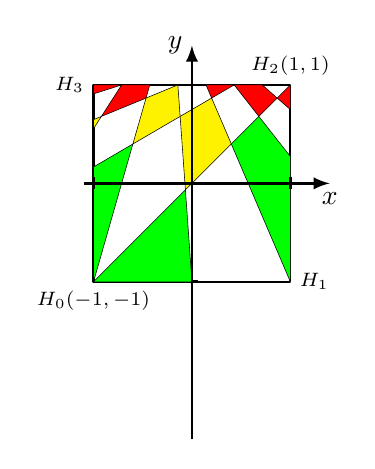
\begin{tikzpicture}[line join=round,line width=0.2pt,>=latex]
\filldraw[fill=none,line width=0.75pt](5.75,-13.25)--(8.25,-13.25)--(8.25,-10.75)--(5.75,-10.75)--cycle;
\filldraw[fill=yellow](6.417,-10.917)--(6.25,-11.5)--(6.85,-11.15)--(6.821,-10.75)--cycle;
\filldraw[fill=red](5.75,-10.75)--(5.75,-10.864)--(6.107,-10.75)--cycle;
\filldraw[fill=red](6.107,-10.75)--(5.85,-11.15)--(6.417,-10.917)--(6.464,-10.75)--cycle;
\filldraw[fill=red](8.25,-11.063)--(8.25,-10.75)--(8.083,-10.917)--cycle;
\filldraw[fill=red](7.85,-11.15)--(8.083,-10.917)--(7.893,-10.75)--(7.536,-10.75)--cycle;
\filldraw[fill=red](7.179,-10.75)--(7.25,-10.917)--(7.536,-10.75)--cycle;
\filldraw[fill=yellow](6.917,-12.083)--(7.5,-11.5)--(7.25,-10.917)--(6.85,-11.15)--cycle;
\filldraw[fill=yellow](5.85,-11.15)--(5.75,-11.306)--(5.75,-11.191)--cycle;
\filldraw[fill=green](8.25,-13.25)--(8.25,-11.659)--(7.85,-11.15)--(7.5,-11.5)--cycle;
\filldraw[fill=green](5.75,-13.25)--(6.25,-11.5)--(5.75,-11.792)--cycle;
\draw[line width=1pt](8.25,-11.925)--(8.25,-12.075);
\draw[line width=1pt](7.075,-13.25)--(6.925,-13.25);
\draw[line width=1pt](7.075,-10.75)--(6.925,-10.75);
\draw[line width=1pt](5.75,-11.925)--(5.75,-12.075);
\filldraw[fill=green](5.75,-13.25)--(7,-13.25)--(6.917,-12.083)--cycle;
\draw[->,line width=1pt](7,-15.25)--(7,-10.25);
\draw[->,line width=1pt](5.625,-12)--(8.75,-12);

    \coordinate [label=below:$x$] (X) at (8.75,-12);
    \coordinate [label=left:$y$] (Y) at (7,-10.25);
  
    \coordinate [label=270:{\scriptsize$H_0(-1,-1)$}] (p0H) at (5.75,-13.25);
    \coordinate [label=  0:{\scriptsize$H_1$}]        (p1H) at (8.25,-13.25);
    \coordinate [label= 90:{\scriptsize$H_2(1,1)$}]   (p2H) at (8.25,-10.75);
    \coordinate [label=180:{\scriptsize$H_3$}]        (p3H) at (5.75,-10.75);
  \end{tikzpicture}% End sketch output
